



















\documentclass[pdflatex,11pt]{aghdpl}
% \documentclass{aghdpl}               % przy kompilacji programem latex
% \documentclass[pdflatex,en]{aghdpl}  % praca w języku angielskim
\usepackage[polish]{babel}
\usepackage[utf8]{inputenc}

% dodatkowe pakiety
\usepackage{enumerate}
\usepackage{listings}
\lstloadlanguages{TeX}

%TODO w każdym rozdziale krótki wstęp co się w nim będzie znajdować
%TODO sprawdzić czy we wstępie są cele pracy - szybkie prototypowanie i zastosowania tworzonego modelu, ewakuacja ludzi itd
% We wstępie TEZA + dokładniejszy opis kolejnych rozdziałów
%[DONE Wąs ma pogrubienia jedynie przy wymienianiu definicji w punktach. Pogrubione nazwy def] pozamieniać pogrubienia na pochylenia. pogrubienia głupio wyglądają. sprw. jak ma dr.Wąs u siebie


%---------------------------------------------------------------------------

\author{Dorota Wojtałow, Jacek Złydach}
\shortauthor{D. Wojtałów, J. Złydach}
%\shortauthor{M. Szpyrka}

\titlePL{Symulacja rozprzestrzeniania się dymu i ognia w oparciu o niehomogeniczne automaty komórkowe}
\titleEN{Simulation of fire and smoke by using non-homogeneous cellular automata}
%\titleEN{Thesis in \LaTeX}


\thesistypePL{Praca inżynierska}

\supervisorPL{dr inż. Jarosław Wąs}
\supervisorEN{Jarosław Wąs Ph.D} %% FIXME <--- nie ma być kropki po D ??

\date{2010}

\facultyPL{Wydział Elektrotechniki, Automatyki, Informatyki i Elektroniki}

\acknowledgements{Serdecznie dziękujemy \dots }

%---------------------------------------------------------------------------

\begin{document}

\titlepages

\tableofcontents
\clearpage

\chapter{Wstęp}
\label{cha:wstep}
%TODO refactoring - czemu nie potrafie zrobić pustej linii przed tezą?!?!?!

%wg. strong Wojnickiego 5 pktow które powinny znaleźć się we wstępie:
% 1. Co - przediot, problem pracy
% 2. Jak - metoda, krotko
% 3. Dlaczego - źrodla problemu badawczego
% 4. Po co - implikacje, konsekwencje, walory
% 5. Co w kolejnych rozdziałach
\section{Temat pracy} % 1 Co

Tematem pracy jest stworzenie symulacji rozprzestrzeniania się dymu i ognia 
w opraciu o niehomogeniczne automaty komórkowe. Zakres pracy obejmuje stworzenie symulacji rozchodzenia się dymu i ognia na podstawie automatów komórkowych wraz z jej wizualizacją, a także walidację stworzonego modelu. 
Celem pracy jest pokazanie możliwości niehomogenicznych automatów komórkowych jako narzędzia umożliwiającego 
odzwierciedlenie rzeczywistego rozprzestrzeniania się dymu i ognia podczas pożaru. 

\section {Geneza tematu} %3 i 4 - Dlaczego i po co

W dobie wszechobecnej urbanizacji i ciągłego budownictwa, wraz ze wzrostem świadomości dotyczącej bezpieczeństwa
pożarowego oraz zaangażowania w jego zagwarantowaniu pojawiła się potrzeba możliwości modelowania i obserwacji rozprzestrzeniania się ognia w zamkniętych budynkach.
Wspomniane symulacje pożarów wykazują szereg zastosowań. Są z powodzeniem wykorzystywane w śledztwach. Dają możliwość odtworzenia przebiegu zdarzeń i porównania z wynikami oględzin. Umożliwiają
zbadanie prototypu budynku pod kątem gwarancji bezpieczeństwa pożarowego. 
Ułatwiają projektowanie systemów oddymiania. W połączeniu z modelami ewakuacji ludzi
stanowią kompleksowy system ułatwiający tworzenie bezpiecznych budowli.

W ostatnich latach powstał szereg programów umożliwiających wizualizcję symulacji rozchodzenia ognia. Opracowane dotychczas rozwiązania swoje działanie 
opierają na metodach numerycznej dynamiki płynów (ang. Computational Fluid Dynamics). Niewątpliwą zaletą numerycznego podejścia jest dokładność wyników. 
Głównymi wadami jest złożoność obliczeń i stopień komplikacji modelu. 
Niehomogeniczne automaty komórkowe umożliwiają znaczne uproszczenie modelu. Uproszczenie modelu powoduje z kolei redukcję złożoności
obliczeń czyniąc automaty komórkowe szczególnie dogodną metodą w przypadku tworzenia prototypów oraz symulacji czasu rzeczywistego.

%dopisać coś jeszcze o tym, że nie ma takich symulatorów wyk. automaty komórkowe 



\textbf{Teza} Wykorzystując zasady tworzenia automatów komórkowych oraz w oparciu o prawa fizyki można w realistyczny sposób
przy użyciu niehomogenicznych 
automatów komórkowych
zamodelować zjawiska rozchodzenia się ognia i dymu podczas pożaru.

W celu wykazania powyższej tezy przeprowadzono następujące działania:
\begin{itemize}
\item Przeprowadzono badania dotyczące zjawisk fizycznych zachodzących podczas pożaru.
\item Zidentyfikowano czynniki mające kluczowy wpływ na kształt i charakter pożaru.
\item Zaproponowano model niehomogenicznego automatu komórkowego odzwierciedlającego prawa fizyczne.
\item Zaimplementowano opracowany algorytm wraz z wizualizacją wyników oraz możliwością edycji danych wejściowych oraz kontroli symulacji w czasie rzeczywistym.
\item Dokonano weryfikacji jakościowej zaproponowanego modelu.
\end{itemize}

\section {Realizacja projektu} % 2 - jak
Praca została zrealizowana jako wolnostojąca aplikacja komputerowa napisana w języku Java. Do renderowania grafiki trójwymiarowej
zostala użyta biblioteka graficzna Java3D. Aplikacja została przetestowana z wykorzystaniem biblioteki JUnit4. 

\section{Zawartość pracy} % 5 - co w kolejnych rozdziałach Tutaj na pewno trzeba dać odnośniki do rozdziałów a nie tytuły!
Praca składa się z [iluś] rozdziałów. 
W pierwszym rozdziale znajdują się podstawy teoretyczne, związane zarówno z modelowanymi zjawiskami fizycznymi jak i użytym algorytmem.
Rozdział Modele symulacji zawiera propozycje zweryfikowanych modeli rozprzestrzeniania się dymu i ognia zaprojektowanych w oparciu
o niehomogeniczne automaty komórkowe. Rozdział Implementacja przedstawia sposób realizacji projektu, napotkane problemy oraz 
ich rozwiązania. Opisuje możliwości graficznego interfejsu użytkownika oraz sposób korzystania z niego.
 % W podsumowaniu znajduje się podsumowanie.... nie wiem jeszcze jak to ładnie ująć
%cos wiecej o rozdzialach. dopisac jak będa gotowe

%TODO:
%Wstawić rysunek konwekcji narysowany ze screena z Rosenbajgerowymi strzałkami
%Konwekcja, a grawitacja i prawo Archimedesa
\chapter{Teoria}
\label{cha:Teoria}
Kluczowym elementem, niezbędnym do prawidłowego zamodelowania pożaru
jest zrozumienie czym jest ogień oraz poznanie zjawisk jakim podlega. Niniejszy rozdział zawiera
krótki wstęp teoretyczny, przedstawiający zjawiska fizyczne niezbędne do zrozumienia istoty 
pożaru i prawidłowego jego zamodelowania.
\section {Czym jest ogień}
Ogień nie jest substancją.
Ogień powstaje jako produkt reakcji chemicznej zachodzącej między paliwem i tlenem.
Obserwowalną postać ognia, czyli to co widzimy i nazywamy ogniem tworzy światło powstałe w wyniku ruchu rozgrzanego powietrzna.
Jest to jednak tylko jeden z aspektów tego złożonego procesu.
Elementami koniecznymi do powstania i podtrzymania ognia są:
\begin{itemize}
\item tlen
\item paliwo
\item ciepło
\end{itemize}


Paliwem może być ciecz, ciało stałe lub gaz. Samo w sobie paliwo nie ulega spalaniu. 
Paliwo pod wpływem ciepła pochodzącego np. z zapałki lub otrzymanego od innego nagrzanego ciała ogrzewa się. Po osiągnięciu
odpowiedniej temperatury, paliwo ulega procesowi dekompozycji. Jednym z produktów dekompozycji
są opary. W przypadku jednego z najbardziej popularnych paliw - drewna oprócz oparów w wyniku dekompozycji otrzymujemy węgiel i popiół.
Spalanie drewna przedstawia poniższa reakcja \ref{reakcja_spalania}:
\begin {equation}
CH_2O+O_2+heat ->CO_2 + CO + C + N_2 + H_2O
\label {reakcja_spalania}
\end {equation}
Kiedy opary osiągną odpowiednią temperaturę tzw. temperaturę zapłonu (w przypadku drewna wynosi ona ok. $300^\circ C$) oraz gdy ich stężenie
w powietrzu jest odpowiednie może dojść do zapłonu. Do zapłonu dochodzi w wyniku kontaktu z otwartym ogniem, iskrą lub w wyniku osiągnięcia
przez opary temperatury tzn. samozapłonu. Wynikiem zapłonu jest spalanie oparów. Jak widać głównym substratem reakcji spalania są opary powstające w wyniku
ogrzania paliwa. W przypadku niektórych paliw jest to jedyny reagent. Jednym z przykładów jest benzyna, która w wyniku ogrzania w całości zamienia się w opary ulegające spalaniu. W przypadku drewna, poza oparami spalaniu ulega także węgiel. Jest to jednak reakcja bardzo powolna.
Na szczególną uwagę zasługuje fakt wytwarzania energii cieplnej w procesie spalania, co powoduje samoistne podtrzymanie ognia. Płomień będący
wizualną postacią spalania ogrzewa sąsiadujące cząsteczki paliwa, dzięki czemu nie gaśnie.

Bardzo istotnym reagentem w procesie spalania jest tlen. Atomy gazów, oparów powstałych w wyniku podgrzania paliwa w wyniku zapłonu łączą się z tlenem.
Aby mogło dojść do reakcji spalania bardzo ważne jest zachowanie odpowiednich proporcji między substratami reakcji. Lower Explosive Limit (LEL) określa 
minimalne stężenie oparów w powietrzu, konieczne aby mogło dojść do zapłonu. Odpowiednio, Upper Explosive Limit (UEL) oznacza maksymalne stężenie oparów, powyżej
którego nie dojdzie do zapłonu. Przykładowo: dla tlenku węgla $LEL=12$, natomiast  $UEL=75$, co oznacza w powietrzu musi być między $12\%-75\%$ aby mogło dojść
do jego zapalenia. $LEL$ oraz $UEL$ określają także pośrednio wymaganą ilość tlenu. Dla większości paliw ilość tlenu wymaganego do zapłonu wynosi ok. $15\%$. 

\section {Propagacja ciepła}
Jak zostało wspomniane w rozdziale \ref{Proces spalania} jednym z czynników niezbędnych
do podtrzymania ognia jest ciepło. Ciepło podczas pożaru jest propagowane na trzy różne sposoby:
\begin {itemize}
\item Przewodnictwo
\item Konwekcja
\item Radiacja
\end {itemize}

\subsection {Przewodnictwo}
\label{Przewodnictwo}
 Przewodnictwo cieplne jest procesem, który polega  na wymianie ciepła 
pomiędzy nierównomiernie ogrzanymi ciałami będącymi w kontakcie. Zachodzi ono we wszystkich stanach skupienia: ciałach stałych, cieczach i gazach, jednak sposób i skala tego zjawiska jest bardzo zróżnicowana. Najczęściej mówimy o przewodnictwie w ciałach stałych.
W cieczach i gazach występuje ono niezmiernie rzadko i polega na zderzeniach cząsteczek podlegających
niezorganizowanym, przypadkowym ruchom i ich dyfuzji.
W ciałach stałych przenoszenie ciepła odbywa się  na dwa sposoby:
\begin{itemize}
\item dzięki drganiom atomów
\item poprzez ruch elektronów
\end {itemize}
Celem omawianego przewodnictwa jest 
osiągnięcie równowagi cieplnej. Podczas przewodnictwa ciepło jest zawsze przenoszone od
ciała o większej temperaturze do ciała o niższej. Zgodnie z zasadą zachowania energii, głoszącą że w układzie 
izolowanym suma wszystkich energii jest stała, ilość energii uzyskanej przez ciało chłodniejsze jest równa
ilości energii oddanej przez cieplejszy obiekt. Energia przenoszona jest wraz z ruchem cząsteczek wewnętrznych.
Nie wszystkie ciała przewodzą ciepło w takim sam sposób.
Zależność między ilością ciepła przewodzonego przez ciało, a jego zmianą temperatury najlepiej opisuje prawo Fouriera.
Przyjmuje ono następującą postać:
\begin{equation}
 q(r,t)=-k*grad T
 \label{eqn:fourier}
\end {equation}
gdzie:
k - współczynnik przewodzenia ciepła $[W / (m*K)]$
T - temperatura $[K]$
q - natężenie strumienia ciepła  $[W/(m^2)]$
Prawo Fouriera oznacza, że gęstość strumienia ciepła przekazywana w jednostce czasu przez jednostkową powierzchnię 
jest proporcjonalna do gradientu temperatury. Minus we wzorze wynika ze wspominanego wyżej kierunku przepływu ciepła:
od ciała cieplejszego do zimniejszego. Strumień ciepła jest mierzony w kierunku zgodnym z jego przepływem, zatem przyrost
temperatury będzie miał wartość ujemną.


Do dobrych przewodników należą przede wszystkim:
\begin {itemize}
\item metale - do najlepszych należą srebro, miedź, złoto, aluminium
\end {itemize}
Źle przewodzą ciepło:
\begin {itemize}
\item drewno
\item papier
\item ciecze
\item gazy
\end {itemize}
Zła przewodność cieczy i gazów wynika z istoty procesu przewodnictwa w tych stanach skupienia. Za wysoką wartość 
współczynnika przewodnictwa odpowiada ruch elektronów. Dlatego też, we wszystkich dialektrykach wartość ta
przyjmuje wartości z przedziału $[0,001-3][W/(m*K)]$, podczas gdy w metalach może sięgać ona nawet $ 400 [W/m*k]$

Na uwagę zasługuje też fakt, że przewodność metali maleje wraz ze wzrostem ich temperatury.
Tabela \ref {przewodnictwa} zawiera współczynniki przewodnictwa przykładowych materiałów, które zostały wykorzystane przy
testowaniu algorytmu symulacji.
%http://tabelechemiczne.chemicalforum.eu/przewodnictwo_ciala.html
%Dodać do bibliografii tablice fizyczne z których to wzięte
\begin{table}
\begin {center}
\begin{tabular} {|l | c | c|}
\hline
Materiał & Temp. $[C]$ & Wspł. przewodnictwa $[W/(m*K)]$ \\ \hline
Beton & 20 & 0.84-1.3  \\ \hline
Drewno & - & 0.1-0.17  \\ \hline
Szkło crown & 20 & 0.22-0.29  \\ \hline
Azbest & 20 & 0.16-0.37 \\ \hline
Guma wulkanizowana & 20 & 0.22-0.29 \\ \hline
Miedź & 20 & 400 \\ \hline
Stal & 20 & 10 \\ \hline
Ołów & 20 & 30 \\ \hline
Powietrze & 20 & 0.025 \\ 
\hline
\end {tabular}
\caption{Współczynniki przewodnictwa materiałów}
\label{przewodnictwa}
\end{center}
\end {table}
\subsection{Konwekcja}
\label{Konwekcja}
Konwekcja, zwana też unoszeniem lub wnikaniem jest to zgodnie ze szkolną definicją sposób przewodnictwa ciepła polegający na
"unoszeniu pobranej energii cieplnej przez cząsteczki substancji i dzięki swojej wędrówce przekazywaniu
energii innym cząsteczkom". 
jak się znajdzie jakaś inna przystępna definicja to podmienić
Konwekcja zachodzi we wszystkich płynach, czyli zarówno cieczach jak i gazach. Nie zachodzi natomiast w ciałach stałych.
Konwekcja ze względu na połączenie w sobie dwóch zjawisk: 
\begin{itemize}
\item przekazywania ciepła
\item ruchu płynów
\end{itemize}
jest zjawiskiem niezwykle skomplikowanym do teoretycznego ujęcia. Przenoszenie ciepła w konwekcji zachodzi 
wskutek ruchu płynu, tak więc warunkiem niezbędnym do wystąpienia zjawiska konwekcji jest ruch ośrodka.
Można wyróżnić dwa podstawowe typy konwekcji, dzielące zjawisko wnikania ze względu na przyczynę ruchu ośrodka:
\begin{itemize}
\item konwekcja naturalna - w tym przypadku ruch płynu wywołany jest różnicami gęstości substancji znajdujących się w polu grawitacyjnym
\item konwekcja wymuszona - ruch płynu spowodowany jest działaniem urządzeń zewnętrznych (wentylatorów, pomp)
\end {itemize}
Przykładem konwekcji naturalnej jest unoszenie ciepłego powietrzna w pomieszczeniu. 
Ogrzane powietrze zmniejsza swoją gęstość, w wyniku czego unosi się do góry. Jego miejsce wypełnia zimne powietrze, 
które w kolejnym etapie ulega ogrzaniu rozpoczynając kolejny cykl wędrówki powietrza. Ruchy powietrza wywołane zjawiskiem 
konwekcji tworzą tzw. prądy konwekcyjne.
%TODO dodać rysunek konwekcji
 Konwekcja naturalna jest typem konwekcji występującym podczas pożaru. 

\subsection {Radiacja}
\label{Radiacja}
Radiacja, czyli inaczej promieniowanie jest to sposób rozchodzenia ciepła w postaci fal elektromagnetycznych. 
Najważniejszym aspektem przewodnictwa ciepła przez promieniowanie jest możliwość wymiany ciepła między ciałami
nie stykającymi się.
W bardzo niskich temperaturach ilość przekazywanego przy pomocy radiacji ciepła jest tak mała, że zjawisko to może być pomijane.
Wzrost znaczenia promieniowania następuje wraz ze wzrostem temperatury ciał wymieniających ciepło.
Przyjmuje się, że radiacja zachodzi dla ciał o temperaturach wyższych od $0 ^\circ$ Kelvin.
Promieniowanie jest rodzajem wymiany energii, która nie wymaga żadnego nośnika. Każde ciało emituje fale.
W normalnych warunkach większość promieniowania zachodzi przy udziale fal podczerwonych. Należy jednak pamiętać
że w radiacji mogą brać udział także fale świetlne czy ultrafioletowe. Poza emisją promieniowania każde ciało reaguje także
na fale wysyłane przez innych. Dla każdego ciała jesteśmy w stanie określić wartości trzech współczynników opisujących 
reakcję ciała na wiązkę promieniowania. Należą do nich:
\begin {itemize}
\item Absorpcyjność czyli pochłanialność
\item Refleksyjność czyli odbijalność
\item Przepuszczalność
\end {itemize}
Radiacja następuje we wszystkich kierunkach aż  do momentu zablokowania drogi promieni przez ciało pochłaniające je.
Większość ciał stałych o rozmiarach większych od kilku mikrometrów nie przepuszcza promieniowania. Na wspomnianej 
głębokości pod powierzchnią ciała następuje całkowita absorpcja promieniowania cieplnego. Ponadto ciała stałe mogą przepuszczać
fale tylko o określonej długości. Przykładem jest szkło, które przepuszcza jedynie fale świetlne.
Ilość promieniowania emitowanego przez ciała szare można obliczyć ze wzoru \ref{emisyjnosc}
\begin {equation}
\dot{Q_{emit}}=\sigma*\varepsilon*A_{s}*T_{s}^4
\label {emisyjnosc}
\end {equation}
gdzie
\begin{itemize}
\item $\varepsilon \in (0,1)$ - emisyjność powierzchni. $\varepsilon=1$ - dla ciała doskonale czarnego. Określa jak bardzo dane 
ciało jest podobne do ciała doskonale czarnego.
\item $\sigma = 5.67 * 10^-8 [W/(m^2 * K^4]) $ - stała promieniowania
\item $A_{s} [m^2]$ - powierzchnia 
\item $T_{s} [K]$ - temperatura
\end {itemize}
Przeanalizujmy przykład promieniowania między rzeczywistymi obiektami znajdującymi się w pewnym pomieszczeniu np. stół w pokoju.
W przypadku jednej powierzchni zamkniętej w innej (w omawianym przypadku wewnętrzną powierzchnią będzie powierzchnia stołu, natomiast zewnętrzną ściany pokoju) zakłada się, że wewnętrzna powierzchnia "nie opromieniowuje samej siebie".
Innymi słowy całe promieniowania ciała wewnętrznego przechodzi do powierzchni zewnętrznej. W drugim kierunku następuje tylko częściowe
przejście energii z ciała zewnętrznego do wewnątrz. Ponadto, w przypadku gdy otaczająca powierzchnia jest znacząco większa od powierzchni wewnętrznej i obie powierzchnie są oddzielone gazem, który nie promieniuje (powietrze) zjawisko promieniowania zachodzi
równolegle ze zjawiskiem konwekcji i oba te zjawiska należy wziąć pod uwagę równocześnie.
W takim przypadku wymianę ciepła można określić za pomocą wzoru \ref{emisyjnosc_konwekcja}
\begin {equation}
\dot{Q_{całk}}=\alfa_{całk}*\sigma*A_{s}*(T_{s}^4-T_\inf^4)
\label {emisyjnosc_konwekcja}
\end {equation}
gdzie:
\begin {itemize}
\item \alfa_{całk} - całkowity współczynnik wymiany ciepła
\item T_\inf - temperatura powietrza w znacznej odległości
\end {itemize} 
Omówione powyżej procesy powodują, że promieniowanie jest zjawiskiem szczególnie skomplikowanym.

\subsection {Zależność temperatury od dostarczonej energii}
Opisane w podrozdziałach \ref{Przewodnictwo}, \ref{Konwekcja}, \ref{Radiacja} metody obrazują różne sposoby przekazywania energii
między cząsteczkami materii. Po ich poznaniu należy zadać sobie pytanie w jaki sposób ta energia wpływa na temperaturę substancji?
Wielkością reprezentującą zależność między dostarczoną energią a temperaturą substancji jest ciepło właściwe. Ciepło właściwe
jest wielkością charakterystyczną dla materiału i  informuje ono o tym ile ciepła
należy dostarczyć aby ograć 1kg substancji o $1^\circ C$.Opisaną powyżej zależność przedstawia wzór \ref{cieplo_wlasciwe} 
\begin {equation}
c=Q/(m*\Delta T)
\label {cieplo_wlasciwe}  
\end {equation}
gdzie:
\begin {itemize}
\item c - ciepło właściwe $[J/ (kg * K)]$
\item m - masa ciała $[kg]$
\item T - temperatura  $[K]$
\end {itemize}
Znając ilość ciepła dostarczonego do ciała w wyniku procesów przekazywania energii oraz dokonując przekształcenia powyższego wzoru
można w bardzo prosty sposób policzyć zmianę temperatury badanego ciała.


%TODO dopiac podział automatów komórkwoych głownie homogeniczne i niehomogeniczne
\chapter{Automaty komórkowe}
\label{cha:Automaty komórkowe}
W rozdziale tym wyjaśniono pojęcie automatu komórkowego, przedstawiono formalną definicję automatów komórkowych oraz ich najczęstsze  zastsowania. Podczas omawiania automatów zamieszczono ogólny algorytm symulacji z wykorzysaniem automatów komórkwoych. Zasadę działania prostych automatów przedstawiono
na przykładzie gry Life. Szczególną uwagę podczas opisu 
 automatów komórkowych poświęcono niehomogenicznym automatom komórkowym, gdyż to one zostały wykorzystane
do symulacji pożaru. 
\section {Definicja automatu komórkowego}
Według definicji \textbf {Ferbera} \textsl{ Automat komórkowy jest dyskretnym, dynamicznych systemem, którego zachowanie jest
całkowicie określone w warunkach lokalnyc relacji.}
Inną definicją, ukazującą automat komórkowy w matematycznym zapisie jest definicja \textbf{Weimara}, przedstawiająca
automat jako czwórkę parametrów:
\begin{Center}
$CellularAutomata=(L,S,N,f)$
\end{Center}
gdzie
\begin{itemize}
\item L - zbiór komórek tworzących automat
\item S - zbiór stanów, które może przyjmować komórka
\item N - zbiór sąsiadów danej komórki
\item f - funkcja przejścia, która każdą komórkę ze zbioru L przeprowadza  ze stanu $S_i$ w stan $S_(i+1)$. $S_t$ jest jednym ze stanów
		ze zbioru S przyjmowanym przez komórkę w i-tej jednostce czasu, natomist $S_(i+1)$ jest stanem przyjmowanym
		przez komórkę w i+1-ej jednostce czasu na podstawie analizy stanów sąsiadów komórki (N).
\end{itemize}
Innymi słowy, automat komórkowy jest to model matematyczny opisujący siatkę komórek, ich stany oraz reguły przejść
między kolejnymi stanami. Każda komórka z pewnej dyskretnej siatki komórek może przyjmować jeden z określonego zbioru stanów.
W dyskretnych przedziałach czasowych następuje ewolucja komórki, na podstawie jej \textbf{stanu poprzedniego} oraz \textbf{stanu jej sąsiadów}. Ewolucję komórki określa funkcja przejścia. Odpowiedni dobór zbioru stanów oraz funkcji przejść kształtuje cechy automatu, jego dynamikę oraz szybkość.
W wyniku ewolucji komórka przyjmuje kolejny stan ze zbioru S. Ze względu na wielwymiarowość automatów komórkwoych, sąsiedztwa można
definiować w różny sposób. W przypadku dwuwymiarowego automatu najprostszym sąsiedztwem, zwanym też sąsiedztwem von Neumana będzie
zbiór czterech komórek {N,S,E,W} gdzie kolejne literki oznaczają kierunki zgodne z różą wiatrów. W dwuwymiarowych automacie jako sąsiedztwo można przyjmować także zbiór ośmiu komórek (sąsiedztwo \textbf{Moore'a}: cztery wspomniane powyżej kierunki wraz z kierunkami pośrednimi {N, S, E, W, NW, NE, SE, SW}. W trójwymiarowym automacie najprostszym sąsiedztwem jest zbiór wszystkich 
komórek połączonych ścianami z aktualnym sześcianem. Innym sąsiedztwem mogą być wszystkie szcześciany połączone z aktualnie badanym
zarówno ścianami jak i krawędziami. Ważnymi elementami automatu komórkowego jest stan początkowy automatu, czyli z góry określony
stan każdej komórki w chwili 0 (przed pierwszą iteracją algorytmu). W przypadku automatów komórkwoych o ograniczonej siatce konieczne
jest także zdefiniowanie warunków brzegowych. Warunki brzegowe określają reguły przejść dla komórek znajdujących się na brzegach
automatu. W przypadku jednowymiarowej siatki, przykładem warunku brzegowego jest określenie sąsiadów ostatniego $n-tego$ elementu jako 
$n-1$ oraz $1$ - przedostatni oraz pierwszy element.
Poniżej przedstawiono ogólny schemat działania algorytmu komórkowego: \\\\
\begin{center}
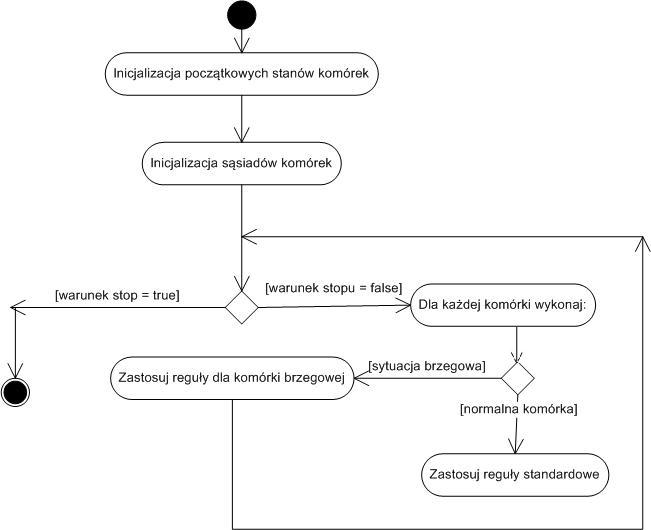
\includegraphics{algorytm_automatu_kom}
\end{center}
\\\\
Automaty komórkowe dzięki możliwościom zastąpienia bardzo skomplikowanych wzorów prostymi regułami są szeroko stoswane do modelowania
procesów fizycznych i chemicznych np. symulacje pożarów lasów, budynków, rozprzestrzenianie lekarstw w organizmie ludzkim. 
Innym zastosowaniem jest symulacja zjawisk, które ze względu na swoją naturę, w wyniku braku zjaomości
dokladnych wzorów nie mogą być odzwierciedlone w sposób dokłady. Przykładem takiej symulacji jest na przykład ruch ludzi podczas ucieczki z ewakuowanego budynku.
\section{Klasyfikacja automatów komórkowych}
Od wprowadzenia pojęcia automatu komórkowego, które datuje się na lata 40-ste XX-go wieku powstały różne metody klasyfikacji automatów komórkowych. Jedną z najważniejszych jest podział ze względu na homogeniczność automatu.
\textbf{Homogenicznym automatem komórkowym} nazywamy, automat który spełnia wszystkie postulaty homogeniczności.
Należa do nich:
\begin{itemize}
\item jednakowy zbiór stanów dla każdej komórki
\item jednakowy zbiór reguł dla każdej komórki
\item stały obszar siatki automatu
\item jednakowy schemat określający sąsiadów dla każdej komórki
\item jednakowa metoda aktualizacji wszystkich komórek
\end {itemize}


Jeżeli automat nie spełnia, \textsl {któregokolwiek} z wyżej wymienionych warunków jest klasyfikowany jako \textbf {niehomogeniczny
automat komórkwowy}. 

Najprostszym przykładem klasycznego, homogenicznego automatu komórkowego jest gra \textsl{Life}. 
W grze Life mamy zazwyczaj do czynienia z nieskończoną planszą Każda
z komórek siatki może przyjmować dwa stany: jest żywa lub martwa. Każda z komórek posiada ośmiu sąsiadów - są to komórki przylegające krawędziami i rogami.W grze tej wszystkie komórki zmieniają swój stan, co pewien ustalony odstęp czasu. Nowy stan komórki jest oblicznay
wyłącznie na podstawie jej poprzedniego stanu oraz stanów sąsiadów. Metoda aktualizacji komórek oraz schemat określający nowy 
stan jest identyczny dla wszystkich komórek automatu. Mimo nazwy omawianej symulacji jedynym udziałem człowieka w tej grze jest
ustawienie stanu początkowego komórek.

Innymi sposobami klasyfikacji automatów komórkowych jest podział ze względu na sąsiedztwo (sąsiedztwo Moore'a oraz von Neumana), 
ze względu na wielowymiarowość planszy (jedno-,dwu-,trój-wymiarowa,...), a także ze względu na kształt pojedynczej komórki.
W jednowymiarowym automacie komórką jest odcinek, w dwuwymiarowym najprotszym wariantem jest kwadrat, a w trójwymiarowej sześcian.
Różnie między tymi automatami zostały częściowo omówione w rozdziale poprzendim.


\end {Center}
\chapter {Projekt}
\label{cha:projekt}
\section {Główne zalożenia}
\begin {itemize}
\item Głównym celem projektu jest stworzenie i weryfikacja modelu rozprzestrzeniania się ognia wykorzystując niehomogeniczne automaty
komórkowe. Nacisk z pracy został położony na opracowanie algorytmu najdokładniej oddającego rzeczywistość.
\item Projekt obejmuje także swtworzenie uproszczonej wizualizacji symulacji oraz graficznego interfejsu użytkownika (GUI).
\item Interfejs aplikacji powinien umożliwiać edycję budynku w którym przeprowadzana jest symulacja: dodawanie elementów konstrukcji, 
określanie materiałów z których zostały stworzone. 
\item Użytkownik powinien mieć możliwość określenia źródła ognia: zarówno jego miejsca jak i temperatury początkowej.
\item Aplikacja powinna umożliwiać także kontrolę nad symulacją: możliwość zatrzymania symulacji, wznowienia, rozpoczęcia od początku,
a także dostosowanie tempa symulacji umożliwiającego obserwację zjawisk fizycznych.
\end {itemize}
\section {Architektura aplikacji}
% w bibliografi powinno byc coś o tej architekturze i def. aktywnego modelu
Aplikacja została zaprojektowana zgodnie z architekturą Model-View-Controller.
Poniższy schemat przedstawia typowy przykład architektury Model-View-Controller:
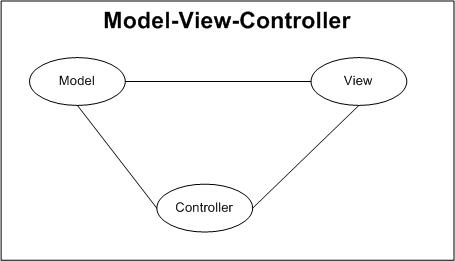
\includegraphics{MVC.jpeg}
W omawianej pracy została zaimplementowana pewna odmiana typowej architektury Model-Widok-Kontroler.
Najodpowiedniej przedstawia ją poniższy rysunek:
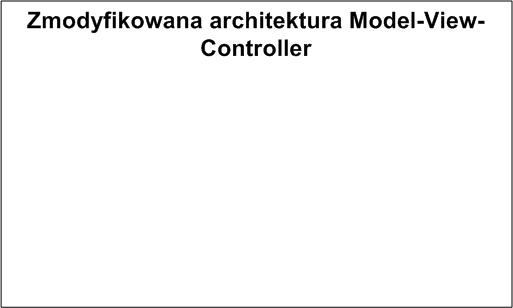
\includegraphics{modifiedMVC.jpeg}
Kontroler odpowiada za pobranie danych od użytkownika, ich przetworzenie oraz dostarczenie do modelu.
Został zastosowany przypadek aktywnego modelu, który zgodnie z definicją potrafi zmieniać swój stan 
bez względu na akcje wykonywane przez użytkownika. W projekcie symulacji pożaru aktywność modelu polega na 
wykonywaniu pętli symulacji, związanych z nią obliczeń, powiadamianiu widoku o zachodzących zmianach oraz
końcu symulacji. Widok odpowiada jedynie za prezentację wyników symulacji.
Wybrana architektura umożliwia elastyczny rozwój aplikacji. Wprowadzony podział na trzy odrębne moduły pozwala
na nieograniczone zmiany w każdym z nich, nie powodując konieczności zmian innych części aplikacji.
Inną zaletą separacji jest łatwość testowania poszcególnych modułów osobno. 
\section {Moduły}
\section {Obiekty}

%TODO dopisać coś wiecej dlaczego mniejsze komórki nie są potrzebne.
% skala  budynku to że nie interesue nas jak dokładnie będzie się palić każde 10cm^3 ale 
% jak ogien będzie się przemieszczał. rozmiar człowieka z perełe
%TODO w sekcji gdzie będzimy sie chwalić wynikami algorytmu napisać o zasadzie zachowania energii
\chapter{Algorytm}
\label{cha:Algorytm}
Rozdział przedstawia propozycję algorytmu symulacji rozprzestrzeniania się ognia i dymu podczas pożaru.
Przedstawiony poniżej model jest niehogenicznym automatem komórkowym i jako taki spełnia postulat niehomogeniczności.
W pierwszej części rozdziału przedstawiono wartości parametrów tworzących automat komórkowy. Kolejne podrozdziały 
zawierają szczegółowy opis kluczowych funkcji współtworzących funkcję przejścia.
% Plan rozdziału
% 1. Jaki typ automatu 3D. wielkość - określana przez usera
% 2. Kształt komórek i wielkość komórek
% 3. Sąsiedztwo - nieregularne, inni sąsiedzi przy krawedziach
% 4. Zbiór stanow
% 5. Funkcja przejscia
% 6. W kolejnych podrozdziałach funkcje będące czynnikami funkcji przejścia - przewodnictwo, konwekcja, dym
% 7. Rodzaje komórek. problem wąskich drzwi i jego rozwiązanie
\section {Model automatu}
Zgodnie ze wzorem \ref{def_automatu} będącym istotą przytoczonej w rozdziale \ref{cha:Automaty komórkowe} definicji automatu komórkowego według Weimara jednym z kluczowych elementów jest określenie siatki, czyli powierzchni automatu. W modelu symulaci pożaru w budynku
ze względu na trójwymiarowość zjawiska oraz istotę jego rzeczywistego odtworzenia (możliwość wykorzystania wyników w celu
opracowania modelu ewakuaci osób, badanie przyczyn katastrofy i drogi rozchozenia ognia) nabardziej naturalnym typem automatu 
jest automat \textsl {trójwymiarowy}. 
Rozmiar automatu jest wielkością zmienną, definiowaną przez użytkownika systemu. Pozwala to na odpowiedni dobór ilości komórek w zależności od wielkości rozpatrywanego budynku. Ze względu na fakt, że istotą przedstawionego modelu jest symulacja pożaru wewnątrz budynku 
Zastosowany twójwymiarowy automat składa się z szcześciennych komórek o wymiarach $0.5m x 0.5m x 0.5m$. Wielkość komórek została wybrana empirycznie. 
Odpowiedni dobór wielkości komórek automatu ma kluczowy wpływ na jego działanie. Zbyt mała ilość komórek może doprowadzić do utraty
dokładności algorytmu oraz ukazać zniekształcony obraz działania modelu. Zbyt duża ilość elementów powoduje spadek wydajności algorytmu, a w komputerowej realizacji algorytmu oznacza zwiększone zapotrzebowanie na pamięć i moc procesora.
Wybrany na podstawie doświadczeń rozmiar komórki jest najlepszym
kompromisem między między czasem działania a dokładnością modelu.
\chapter {Implementacja}
\label{cha:implementacja}
Poniższy rozdział zawiera przegląd ciekawszych aspektów implementacyjnych projektu.
Na wstępie omówiono użyte technologie oraz narzędzia wraz z uzasadnieniem wyboru. Następnie przedstawiono dokładny model aplikacji z uwzględnieniem wybranych metod implementacyjnych. 
W rozdziale tym przedstawiono także problemy, z którymi zetknęli się autorzy podczas realizacji projektu oraz sposoby ich rozwiązania.
\section {Wybrane technologie i narzędzia}
Przed przystąpieniem do implementacji końcowej wersji aplikacji powstawały prototypy testujące różne podejścia algorytmiczne opisane w rozdziale \ref{cha:Algorytm} oraz możliwe do wykorzystania narzędzia. W sekcji \textit{Język implementacji} przedstawiono język wybrany do implementacji końcowej wersji programu, natomiast w sekcji \textit{Języki prototypowania} przedstawiono technologie używane do tworzenia prototypów systemu. 
W kolejnych podrozdziale pokrótce zaprezentowano narzędzia pracy grupowej wykorzystywane przez autorów pracy. Na końcu wymieniono biblioteki i narzędzia, które okazały się pomocne podczas realizacji projektu Sparkle i które zostaną szczegółowo omówione w kolejnych rozdziałach.
\subsection{Język implementacji}
Do implementacji końcowej wersji aplikacji został wybrany język Java.
Język ten został wybrany ze względu na przenośność aplikacji, obiektowość ułatwiającą projektowanie, dostęp do licznych 
bibliotek oraz mechanizmy pozwalające uchronić program przed wyciekami pamięci krytycznymi z punktu widzenia aplikacji czasu rzeczywistego. Innym, rozważanym językiem implementacji był język C++. Przed końcowym wyborem zostały przeprowadzone badania dotyczące wydajności rozważanych języków. Przyniosły one następujące rezultaty:
%http://java.sun.com/docs/performance/ - może z tego uda się coś wyciągnąć o efektywności javy
\begin{itemize}

\end{itemize}

\subsection{Języki prototypowania}
Jednym z powstałych ptotypów był prosty automat komórkowy z regułami opisanymi w paragrafie [WSTAWIC ODNOSNIK DO PARAGRAGU]. Do implementacji tego modelu został korzystany język Common Lisp.

Common Lisp to nowoczesny dialekt Lispu - drugiej najstarszej rodziny używanych obecnie wysokopoziomowych języków programowania. Common Lisp jest językiem kompilowalnym, dynamicznie typowanym i umożliwia tworzenie na znacznie wyższym poziomie abstrakcji niż C++ czy Java. Samo programowanie w tym języku opiera się głównie o stopniową rozbudowę działającego obrazu programu poprzez REPL (ang. Read-Eval-Print Loop) - pętlę tworzącą swoisty interpreter, pozwalającą modyfikować, dokompilowywać i wymieniać fragmenty kodu w czasie działania samego programu. Te wszystkie cechy języka Common Lisp tworzą z niego idealne narzędzie do szybkiego prototypowania programów. Istotnie, omawiany prototyp automatu komórkowego powstał w przeciągo około dziesięciu godzin.

Drugim, powstałym podczas badań pierwowzorem był program napisany w języku Java.
Celem tego modelu było przetestowanie języka Java oraz biblioteki Java3D pod kątem możliwości wykorzystania do implementacji symulacji czasu rzeczywistego w oparciu o uproszczony model automatu. 

\subsection {Narzędzia pracy grupowej}
Ze względu na fakt, że omawiana aplikacja powstała jako wynik pracy dwuosobowego zespołu, bardzo przydatnym narzędziem okazał się system kontroli wersji. Jako system zarządzania wersjami został wybrany Git.
Git jest darmowym, rozproszonym systemem, opartym na architekturze peer-to-peer. W przeciwieństwie do scentralizowanych odpowiedników (np. SVN) nie posiada jednego, centralnego repozytorium z którym członkowie zespołu synchronizują swoje zmiany ale całkowicie niezależne repozytoria, które można synchronizować w różnorodny sposób.

Git, będąc rozproszonym systemem kontroli wersji, posiada dwie istotne cechy kluczowe dla rozwoju niniejszej pracy. Po pierwsze, techniczna równorzędność wszystkich kopii repozytoriów pozwoliła na bezpieczny i niezależny rozwój projektu nawet w sytuacjach, gdy komputer odłączony był od sieci Internet. Możliwość niezależnej pracy na lokalnych repozytoriach skutecznie zachęca do rejestrowania w systemie kontroli wersji nawet drobnych zmian, gdyż synchronizację pomiędzy poszczególnymi developerami można odłożyć do stosownego momentu. Drugą ważną właściwością Gita jest łatwość, z jaką łączy on zmiany wprowadzone przez rózne osoby w tym samych plikach (ang. "merging"). Brak problemów z łączeniem różnych ścieżek rozwoju - problemów znanych z tradycyjnych, centralnych systemów kontroli wersji - pozwolił na szybki rozwój projektu.

\subsection{Inne narzędzia}
\begin{enumerate}
\item Implementacja prototypu w Common Lisp została oparta o edytor Emacs oraz biblioteki SDL i OpenGL.
% FIXME prototyp a projekt
\item Do implementacji projektu zostały wykorzystane środowiska programistyczne: Eclipse i NetBeans. Użycie systemu kontroli wersji do wymiany plików źródłowych aplikacji dało możliwość niezależniej pracy w różnych środowiskach.
\item Podczas realizacji Graficznego Interfejsu Użytkownika został wykorzystany program WindowBuilder Pro.
\item Wizualizacja symulacji została zaimplementowana z wykorzystaniem biblioteki Java3D.
\item Metody tworzące algorytmikę aplikacji zostały przetestowane z wykorzystniem biblioteki JUnit4.
\item Do badania pokrycia kodu testami jednostkowymi zostało wykorzystane narzędzie Emma.
\end{enumerate}


\section {Implementacja modelu aplikacji}
Zgodnie z architekturą aplikacji omówioną w rozdziale \ref{cha:projekt} program został podzielony na 
\begin{itemize}
\item Moduł wizualizacji danych
\item Moduł realizujący logikę aplikacji
\item Moduł kontrolera, odpowiadający za interakcje z użytkownikiem.
\end{itemize}
Poniżej przedstawiono najważniejsze implementacyjne aspekty realizacji poszczególnych modułów.
Opis implementacji wzbogacony został o diagramy klas UML przedstawiające budowę poszczególnych pakietów, zwracające uwagę na powiązania między jednostkami oraz uwypuklające wybrane metody implementacyjne.
\subsection {Moduł wizualizacji}
Wizualizacja symulacji została zaimplementowana z wykorzystaniem Java3D API.
Java3D to interfejs programowy (API) umożliwiający tworzenie trójwymiarowej grafiki. Jest to produkt firmy Sun Microsystems wykorzystujący w swoim działaniu renderery OpenGL i Direct3D w zależności od platformy.
Główną zaletą determinująca wybór bilioteki Java3D jest umożliwienie wykorzystania technologii OpenGL i DirectX poprzez dostarczenie wysokopoziomowych struktur pozwalających zachować pełnię obiektowości języka Java. 
Zastosowana w bibliotece Java3D obiektowość ułatwia zarządzanie elementami sceny oraz umożliwia skupienie uwagi na logice aplikacji bez zagłębiania się w szczegóły renderingu. Inną niezmiernie ważną zaletą biblioteki Java3D jest optymalizacja procesów renderingu.
\subsubsection{Instalacja biblioteki Java3D}
Instalacja biblioteki Java3D jest stosunkowo prosta i może przebiegać na dwa sposoby.
Pierwszym sposobem jest ściącienie ze strony 
\begin{center}
https://java3d.dev.java.net/binary-builds.html
\end{center} \\
 archiwum zip. Po jego rozpakowaniu należy, postępując zgodnie z instrukcją zawartą w pliku README-unzip.html, zmodyfikować zmienną CLASSPATH dodając ścieżki do wymienionych w instrukcji plików z rozszrzeniem .jar oraz zmodyfikować zmienną PATH dodając ścieżkę do katalogu lib\i386.


Alternatywą jest pobranie ze strony firmy Oracle 
\begin{center}
http://www.oracle.com/technetwork/java/javase/tech/index-jsp-138252.html \\
\end{center}
instalatora, który pod dwukrotnym kliknięciu przeprowadzi użytkownika przez proces instalacyjny. 
W wyniku instalacji, Java Runtime Environment System Library zostanie wzbogacone o pliki j3dcore.jar i j3dutils.jar.
\subsubsection{Budowa sceny z wykorzystaniem struktur Java3D API}
Głównym elementem biblioteki Java3D jest graf sceny (\textit{scene graph}) rerezentujący cały wirtualny wszechświat (\textit{virtual universe}). Graf sceny jest acyklicznym grafem skierowanym.  Użytkownik tworzy podgrafy reprezentujące pewne wycinki rzeczywistości, które następnie są dołączane jako dzieci do wirtualnego wrzechświata. Kazdy z podgrafów jest renderowany  osobno i niezależnie od pozostałych, co pozwala na zrównoleglenie obliczeń. Strukturę grafu sceny przedstawia diagram \ref{java3d_diagram_sceny}.
\begin{figure}
\begin {center}
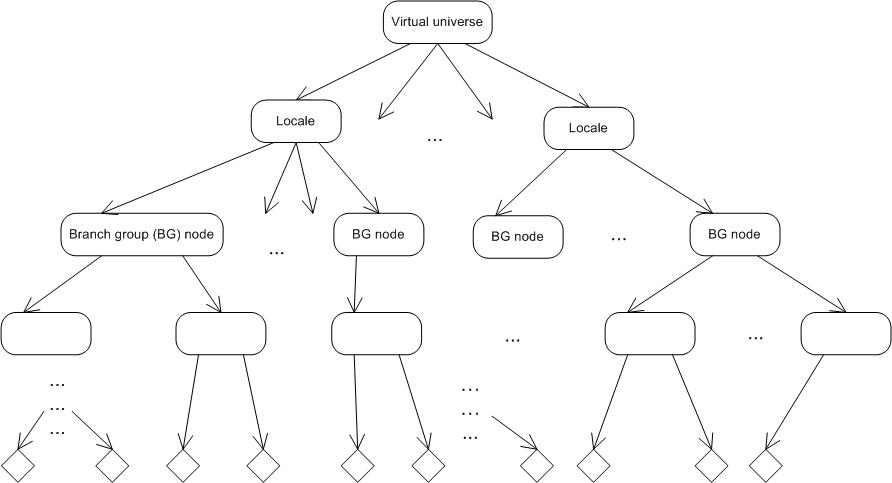
\includegraphics{java3d_diagram_sceny.jpg} 
\caption {Java3D - reprezentacja sceny}
\label {java3d_diagram_sceny}
\end {center}
\end{figure}
 Wśród jego wierzchołków możemy wyróżnić:
\begin{itemize}
\item Group nodes - wierzchołki reprezentujące grupę elementów. Mogą zawierać zero lub więcej dzieci. Grupowanie elementów umożliwia wykonywanie operacji dla całej grupy. Na diagramie \ref{java3d_diagram_sceny} przedstawione są jako zaokrąglone kształty.
\item Leaf nodes - liście reprezentują obiekt tworzący scenę (geometrię, oświtlenie, dźwięk). Nie mogą posiadać dzieci. Na diagramie \ref{java3d_diagram_sceny} występują w postaci rombów.
\end{itemize}
Korzeniem całego grafu jest obiekt klasy \textit{VirtualUniverse} lub dowolnej, dziedziczącej po niej klasie. Graf sceny może posiadać wiele wierzchołków, jednak w większości przypadków jeden jest wystarczający. Obiekt klasy \textit{Locale} jest kontenerem przechowującym kolekcję podgrafów, których korzeniami są instancje klasy \textit {BranchGroup}. Obiekt klasy \textit{BranchGroup} powinien być postrzegany jako jednostka, która po stworzeniu jest kompilowana, a następnie dołączana do grafu reprezentującego wirtualny wszechświat. W dowolnym momencie może zostać odłączana i powtórnie dołączona w inne miejsce.
Tworzenie obiektu 3D przy użyciu Java3D API przebiega następująco:
\begin{enumerate}
\item Tworzony jest obiekt. Ustalane są jego właściwości.
\item Stworzony obiekt dołączany jest do odpowiedniego grafu reprezentowanego przez obiekt BranchGroup.
\item Powstałe grafy w ten sposób grafy są łączone w jedną strukturę reprezentującą wirtualny wszechświat.
\end{enumerate}
Dobrą praktyką jest wspomniane powyżej kompilowanie stworzonych podgrafów przed ich połączeniem. Nie jest ono konieczne ale powoduje  zamianę grafu do wewnętrznego formatu umożliwiającego jego optymalizację. Na uwagę zasługuje fakt, że domyślnie obiekty mogą być modyfikowane jedynie podczas tworzenia podgrafu. Po dołączeniu już stworzonego podgrafu do większej całości informacja o jego obiektach jest oddzielnie zapamiętywana, w sposób przyspieszający operacje dostępu do danych. Można to zmienić wywołując podczas tworzenia obiektu metodę \textit{setCapability} z odpowiednim parametrem.

Przedstawiony powyżej graf sceny jest logiczną reprezentacją renderowanych obiektów.
Do renderingu przygotowanej sceny konieczny jest obiekt klasy Viewer.
Zawiera on wszelkie informacje potrzebne do stworzenia obrazu całej sceny. Z obiektem klasy VirtualUniverse połączony jest
poprzez instancję klasy ViewingPlatform, która inicjalizuje obiekt klasy Viewer dla stworzoneg grafu.
Obiekt klasy Viewer posiada referencje do obiektów klasy View, będących jego lokalnym odpowiednikiem.
Obiekt klasy \text{View} zawiera wszystkie iformacje potrzebne do renderingu pojedynczego elementu sceny oraz referencję do instancji klasy Canvas3D, gdzie opisywany element ma być wyrenderowany.
Jest on połączony z każdym liściem grafu sceny poprzez instancję klasy \textit {ViewPlatform}.
Klasa ViewPlatform odpowiada za inicjalizację obiektu View oraz pozycję, orientację i skalę opisywanego wierzchołka grafu sceny.

\subsubsection{Implementacja modułu wizualizacji}
Moduł wizualizacji zaimplementowany w pakiecie View jest realizacją schematu przedsawionego na diagramie \ref{uml_view}.
\begin{figure}
\begin {center}
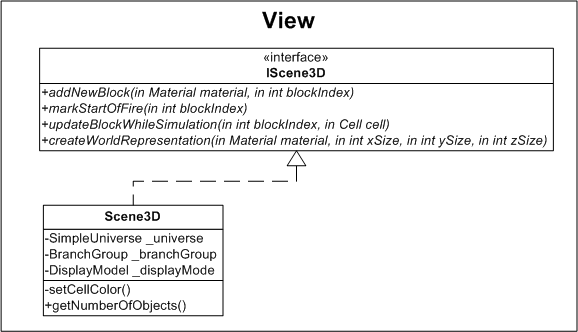
\includegraphics{uml_view.png} 
\caption {Moduł View}
\label {uml_view}
\end {center}
\end{figure}

Klasa Scene3D, implementująca interfejs IScene3D, realizuje przedstawioną powyżej budowę sceny z wykorzystaniem interfejsu Java3D.
Składa się z następujących atrybutów:
\begin{itemize}
\item \_universe - Do budowy korzenia grafu sceny została wykorzystana klasa \textit{SimpleUniverse}. SimpleUniverse pozwala na najprostszą formę inicjalizacji grafu sceny z wykorzystaniem domyślnie tworzonych obiektów klasy \textif{Viewer} oraz \textit{ViewingPlatform}. 
\item \_branchGroup - Obiekt klasy BranchGroup jest podgrafem reprezentującym tworzony budynek. Jest on listą obiektów klasy \textit{TransformGroup}, reprezentujących pojedyncze komórki automatu. Zastosowanie klasy \textit{TransformGroup} umożliwia przemieszczenia poszczególnych
elementów budynku w trakcie działania aplikacji.
\item \_displayMode - DisplyMode odpowiada za tryb wyświetlania wyników symulacji. Może przyjmować jedną z dwóch wartości: TEMPERATURE - powodującą przejście symulacji w tryb wyświetlania rozkładu temperatur podczas pożaru lub REGULAR - przedstawiającą aktualny stan komórki.
\end{itemize}
Interfejs \textot{IScene3D} dostarcza metody umożliwiające wizualizację symulacji. Poniżej przedstawiono ich krótką charakterystykę:
\begin{itemize}
\item \textit{addNewBlock} - dodaje do widoku sceny nowy element knstrukcyjny poprzez zaaplikowanie atrybutów określających wygląd wskazego materiału do określonej przez \textit{blockIndex} komórki. \textif{BlockIndex} jest numerem odpowiadającego elementu z listy \textit{\_branchGroup}. Index jest wyliczany w klasie World, z której wywoływana jest omawiana metoda.
\item \textit{markStartOfFire} - pokazuje źródło pożaru poprzed pokolorowanie odpowiedniej komórki.
\item \textit{updateBlockWhileSimulation} - zmienia wygląd komórki określonej przez \textit{blockIndex} zgodnie z wartościami jej temperatury i materiału oraz uwzględniając aktualny tryb wyświetlania symulacji.
\item \textit{createWorldRepresentation} - tworzy wizualizację automatu komórkowego. Podczątkowy cały automat składa się z komórek wypełnionych tlenem. Metoda \textit{createWorldRepresentation} odpowiada za wypełnienie automatu o wskazanych rozmiarach wytypowanym materiałem (sugerowanym materiałem jest tlen). Tak przygotowany automat możliwy jest do modyfikacji poprzez dodawanie kolejnych elementów konstrukcyjnych lub w wyniku przeprowadzonej symulacji.
\end{itemize}

\subsection {Logika aplikacji}
Logika aplikacji zaimplementowana jest w obrębie pakietu \textit{Model}.
Jego budowę przedstawia diagram \ref{uml_model}.
Diagram klas poza wewnętrzną budową modułu obrazuje jego interakcje z klasami zewnętrznymi, pochodzącymi z innych modułów.
W przypadku Modelu jest to jedynie klasa \textit{Scene3D} z pakietu \textit{View}.
Główną klasą pakietu \textit{Model} jest \itextit{World}. Zawiera ona strukturę danych reprezentującą autmat komórkowy oraz
zestaw metod umożliwiających przeprowadzanie symulacji.
\subsubsection{World}
Klasa World została zaimplementowana jako \textit{Singleton}, ze względu na fakt
jest unikalności w obrębie aplikacji. 

Strukturą danych, która posłużyła do przechowywania automatu jest trójwymiarowa tablica. Innym kontenerem bardzo często wykorzystywanym do reprezentacji przedstawianego świata w symulacjach jest drzewo ósemkowe, którego użycie również zostało rozważone podczas realizacji projektu Sparkle. Poniżej prezentowane są krótkie rozważania na temat wymienionych struktur wraz z uzasdanieniem wyboru. 

Drzewo ósemkowe to strukturą pozwalająca podzielić trójwymiarowy świat na mniejsze, regularne części. Jest ono tworzone zgodnie z następującymi regułami:
\begin{itemize}
\item Korzeniem drzewa jest sześcian, w którym zawarty jest modelowany świat.
\item Każdy z wierzchołków reprezentuje sześcian będący częścią całego obiektu. 
\item Każdy z wierzchołków nie będący liściem posiada osiem dzieci, reprezentujących sześciany w nim zawarte zgodnie z rysunkiem \ref{drzewo_osemkowe}.
\end{itemize}
\begin{figure}
\begin {center}
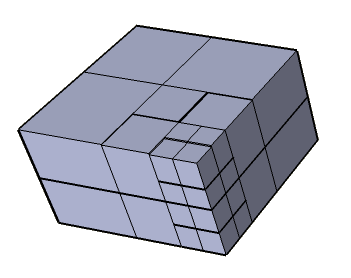
\includegraphics[scale=0.5]{drzewo_osemkowe.png} 
\caption {Podział sceny przy pomocy drzewa ósemkowego}
\label {drzewo_osemkowe}
\end {center}
\end{figure}
Drzewo ósemkowe daje możliwość optymalizacji wykrozystywanej pamięci poprzez przechowywanie jedynie komórek, których stan różni się od stanu rodzica. Komórki identyczne z rodzicem są przez niego reprezentowane, a rodzic taki staje się liściem drzewa. 
Taki sposób przechowania danych jest szczególnie korzystny w przypadku dużej ilości komórek nie biorących udziału w symulacji.
Jest też często wykorzystywany przy renderingu sceny składającej się w znacznej mierze z powietrza, które można zaniedbać.

W przypadku symulacji pożaru, próba adaptacji omawianej struktury okazała się nieefektywna.
Główną przyczyną jest dynamika modelowanego systemu, w którym stan większości komórek zmienia się w krótkim czasie po uruchomieniu symulacji, a kolejne zmiany następują z dużą częstotliwością. Algorytmy propagacji ciepła powodują, że możliwość wyodrębnienia  sześcianu  którego części składowe miałyby stan identyczny z rodzicem należy do rzadkości. Powoduje to, że korzyści płynące ze stosowania wyżej omówionej optymalizacji w przypadku symulacji pożaru są znikome. 
 Bardzo istotnym faktem jest także dodatkowe zużycie pamięci wynikające ze stosowania wskaźnikowej struktury danych. W przypadku gdy drzewo ósemkowe jest drzewem pełnym (każdy z wierzchołków nie będących liściem posiada osiem dzieci) ilość pamięci zużytej przez drzewiastą reprezentajcę przewyższa ilość wykorzystywaną w przypadku implementacji tablicowej.
\begin{figure}
\begin {center}
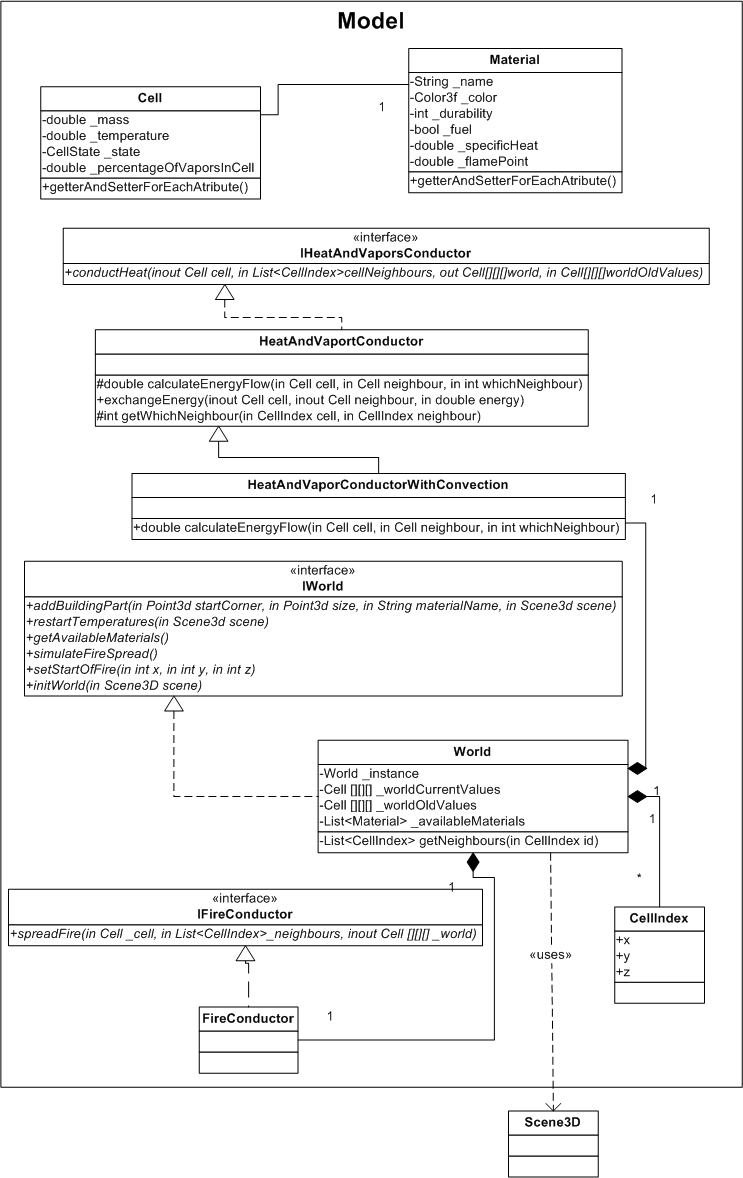
\includegraphics{uml_model.png} 
\caption {Moduł Model}
\label {uml_model}
\end {center}
\end{figure}

Klasa World przechowuje macierz komórek w dwóch egzemplarzach. Podwójne przechowywanie wartości automatu umożliwia odczytywanie parametrów komórki z jednej tablicy, a ich uaktualnianie w drugiej. Taki zabieg nosi nazwę \textit{podwójne buforowanie} czyli \textit{double-buffering} i pozwala uniknąć kierunkowości symulacji. W przypadku nie zastosowania powyższej taktyki temperatura podczas symulacji pożaru rozchodzi się zawsze zgodnie z kierunkiem aktualizacji komórek. Instancja klasy World przechowuje także listę materiałów, które mogą być elementami konstrukcyjnymi budynku. Klasa World zawiera wewnętrzną klasę pomocnicza CellIndex,  która przedstawia index komórki w postaci trzech współrzędnych (x,y,z).

Klasa World impleentuje interfejs IWorld, do którego metod należy:
\begin{itemize}
\item \textit{addBuildingPart} - do odpowiedzialności tej metody należy zmiana materiału komórek wchodzących w skład dodawanego bloku, a także wywołanie odpowiedniej metody klasy Scene3D dokonującej akualizacji widoku podczas edycji budynku. Zadaniem metody addBuildingPart jest zamiana indeksu komórki zapisanego w postaci trójki liczb (x,y,z) na numer odpowiadającej komórki w liście.
\item \textit{restartTemperatures} - metoda wywoływana podczas restartu symulacji. Nadaje wszystkim komórkom parametry domyślne.
\item \textit{getAvailableMaterials} - zwraca listę materiałów, z którym można konstruować budynek.
\item \textit{simulateFireSpread}  - wykonuje jeden przebieg algorytmu aktualizacji automatu komórkowego, wywołując w tym celu metody klas HeatAndVaporConductorWithConvection i FireConducter. Metoda ta jest także odpowiedzialna za wywołanie aktualizacji widoku po każdym przebiegu pętli. Odpowiada za aktualizację macierzy automatu tak aby w każdej chwili macierz, z której czytane są dane była możliwie aktualna z zachowaniem spójności.
\item \textit{setStartOfFire} - ustala punkt startowy pożaru, zmieniając odpowiednio wartości wskazanej komórki.
\item \textit{initWorld} - inicjalizuje autmat wartościami domyślnymi. Domyślnym materiałem wypełniającym przestrzeń jest Tlen. Temperatura komórek na początku działania aplikacji ustawiana jest na $20^\circ C$. Metoda ta odpowiada także, za wywołanie funkcji tworzącej graficzną reprezentację modelu (\textit{createdWorldRepresentation} z klasy \textit{Scene3D}).
\end{itemize}
Ponadto klasa World zawiera metody pomocnicze, do których należy:
\begin{itemize}
\item \textit{getNeighbours} - zwracająca listę indeksów sąsiadów badanej komórki
\item \textit{updateOldValues} - aktualizująca macierz wartości do odczytu
\end{itemize}

\subsubsection{Cell i Material}
To klasy, które zgodnie z opisem zawartym w rozdziale \ref{cha:projekt} zawierają zestaw prywatnych atrybutów określających  odpowiednio stan komórki i właściwości materiału. Z każdym atrybutem związane są metody get i set, kontrolujące dostęp do zmiennych. 

\subsubsection{FireConductor}
Klasa FireConductor odpowiada za rozprzestrzenianie ognia zgodnie z algorytmem opiany w rozdziale \ref{cha:Algorytm}.
Implementuje interfejs IFireConductor zawierający metodę \textit{spreadFire}. Metoda ta jest odpowiedzialna za zmianę stanu komórki
z naturalnego na palący i odwrotnie.

\subsubsection{HeatAndVaporsConductor oraz HeatAndVaporConductorWithConvection}
Do bardziej rozbudowanych klas należy HeatAndVaporsConductor oraz HeatAndVaporConductorWithConvection.
Klasa HeatAndVaporsConductor implementuje interfejs IHeatAndVaporsConductor, definiując metodę \textit{conductHeat}.
Metoda ta wywoływana jest dla każdej komórki automatu, w każdym obiegu algorytmu.
Odpowiada za obliczenie energii przepływającej między badaną komórką i jej wszystkimi sąsiadami oraz symulację wymiany ciepła, 
której wynikiem jest uaktualnienie temperatur komórek. Wszystkie obliczenia przeprowadzane są zgodnie z metodami odpisanymi w rozdziale \textit{Algorytm}. W ich realizacji wykorzystywane są pomocnicze metody: 
\begin{itemize}
\item \textit{calculateEnergyFlow} - odpowiadająca za obliczenie ilości energii przepływającej między dwoma komórkami \\ 
oraz 
\item \textit{exchangeEnergy} - symulująca wymianę ciepła. 
\end{itemize}
Klasa HeatAndVaporsConductor podczas wyliczania przepływającej energii uwzględnia jedynie zjawisko przewodnictwa cieplnego, zaniedbując konwekcję. 

Symulacja konwekcji, jak wyjaśniono w rozdziale \ref{cha:Algorytm} opiera się na ułatwieniu przepływu ciepła do górnych sąsiadów komórki. Konwekcja jest więc szczególnym przypadkiem przewodnictwa, występującym w powietrzu. Zgodnie z powyższym, klasą realizującą konwekcję jest HeatAndVaporConductorWithConvection dziedzicząca po klasie HeatAndVaporsConductor. Przedefiniowana w  klasie potomnej metoda \textit{calculateEnergyFlow} wywołuje odpowiadającą funkcję klasy nadrzędnej, a następnie wprowadza do wyliczonej zgodnie z regułami przewodnictwa energii zmiany wywołane konwekcją. Zmiany te aplikowane są tylko w przypadku gdy badana komórka oraz komórka sąsiednia, z którą następuje wymiana ciepła są powietrzem. Metoda \textit{exchangeEnergy} poza wymianą ciepła między sąsiadującymi komórkami implementuje także przekazywanie drogą konwekcji oparów koniecznych do zapłonu komórki.

\subsection {Moduł obsługi zdarzeń}
Głównym zadaniem modułu obsługi zdarzeń zwanym także \textit{Controllerem} jest obsługa interakcji z użytkownikiem. 
Zgodnie z omówioną w rozdziale \ref{cha:projekt} moduł ten łączy w sobie elementy widoku, tworzące Graficzny Interfejs Użytkownika oraz metody obsługujące wywołane zdarzenia.
Implementacja modułu zawarta jest w pakiecie \textit{Controller}, a jej budowę przedstawia diagram \ref{uml_kontroler}. Adekwatnie do diagramu klas reprezentującego moduł \textit{Model},
ilustracja \ref{uml_kontroler} przedstawia powiązania między klasami modułu \textit{Controller} oraz innymi modułami aplikacji.
\begin{figure}
\begin {center}
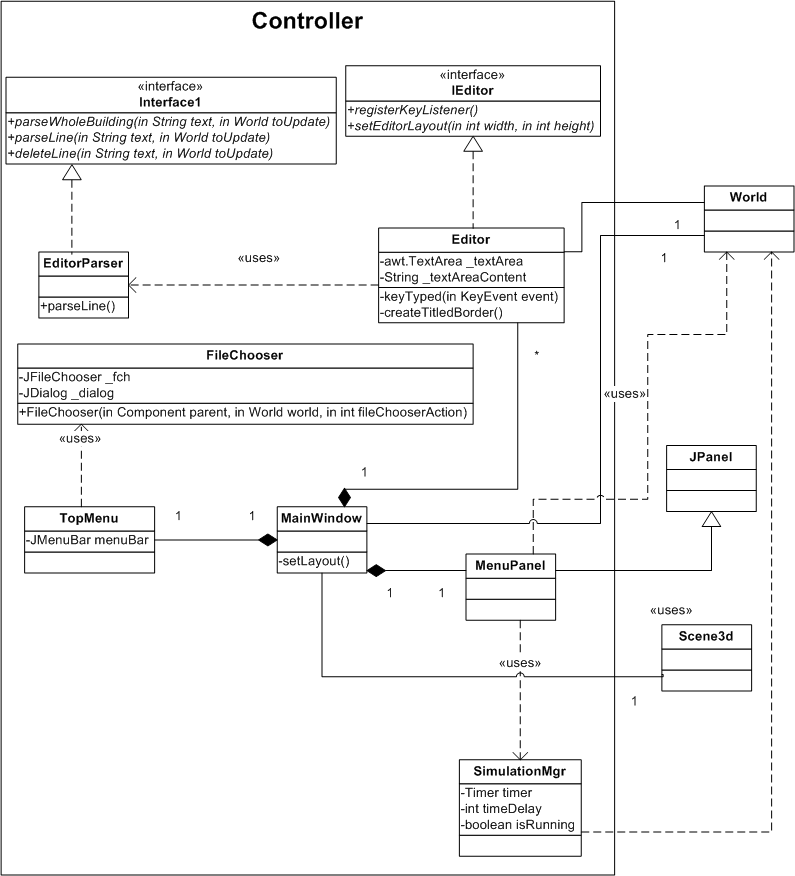
\includegraphics{uml_kontroler.png} 
\caption {Moduł Controller}
\label {uml_kontroler}
\end {center}
\end{figure}
\subsubsection{WindowBuilder Pro - narzędzie do budowy GUI}
Elementy tworząceg GUI zostały stworzone z wykorzystaniem narzędzia WindowBuilder Pro. Jest to darmowe narzędzie, które można zainstalować jako Plugin środowiska Eclipse. WindowBuilder Pro jest edytorem typu WYSIWYG (What You See Is What You Get), pozwalającym na tworzenie graficznych interfejsów użytkownika z wykorzystaniem bibliotek Swing, SWT czy GWT. 

WindowBuilder poza możliwościa tworzenia w łatwy sposób interfejsu aplikacji, umożliwia edycję GUI stworzonego przy pomocy innego oprogramowania. Posiada wbudowany parser, który po otrzymaniu jako argument głównej klasy tworzącej interfejs, przeprowadza analizę kodu i jego wizualizację. Pozwala to na wykorzystanie edytora do poprawy wyglądu aplikacji jednocześnie zachowując przejrzystość kodu w wyniku ręcznej refaktoryzacji.

Innymi przydatnymi cechami wyróżniającymi edytow WindowBuilder Pro jest możliwość tworzenia hierarchii elementów oraz związana z nią
możliwość zamiany typu elementu tworzącego GUI po jego osadzeniu w aplikacji. WindowBuilder umożliwia tworzenie własnych elementów wizualnych dziedzicących po standardowych klasach zawartych w bibliotekach Swing, SWT czy GWT oraz po typach stworzonych przez projektanta. Ta funkcjonalność pozwala na łatwe dostosowywanie komponentów do potrzeb aplikacji oraz dostarcza możliwość tworzenia modułu interfejsu łatwego do utrzymania i modyfkacji.
Druga z wymienionych opcji została nazwana przez autorów programu Morph. Umożliwia ona zamianę obiektu dowolnej klasy na instancję klasy po niej dziedziczącej zgodnie z polimorfizmem oraz instancję klasy podobnej. Do klas podobnych zaliczane są typy posiadające wspólne cechy. W przypadku takiej zamiany zachowywane są właściwości wspólne dla obiektów obu klas. 

\subsubsection{Budowa modułu}
Poniżej została przestawiona implementacja poszczególnych klas wchodzących w skład modułu.
\subsubsection {MainWindow}
Jest to główna klasa modułu Controller i jednocześnia główna klasa aplikacji, zawierająca metodę main.
 W konsturktorze obiektu tworzone są 
elementy składowe głownego okna, do których należą obiekty klas:
\begin{itemize}
\item {MenuPanel}
\item {TopMenu}
\item {Editor}
\item {Scene3D}
\end{itemize}
Klasa MainWindow zawiera także referencję do obiektu typu World, który jest aktualizowany w czasie symulacji.
Konstruktor odpowiada także za rejestrację metod obsługujących zakończenie działania aplikacji.
W  prywatnej metodzie \textit{setLayout}, która jest wywoływana podczas konstrukcji okna, ustalane jest rozmieszczenie jego elementów składowych. Zastosowanym sposobem rozmieszczania jest \textit{BorderLayout}, który pozwala na elastyczne dopasowywanie rozmiaru komponentów do aktualnej wielkości okna.
\subsubsection{MenuPanel}
MenuPanel jest klasą, która pozwala na sterowanie symulacją oraz pozwala na dodawanie elementów konstrukcyjnych budynku.
Zbudowana jest z dwóch obiektów klasy JPanel odpowiadających zakładkom Simmulation i AddingNewBlocks. Wszystkie elementy składowe paneli(pola tekstowe, etykiety, guziki) będące również atrybutami klasy MenuPanel zostały stworzone z wyłącznym wykorzystaniem biblioteki Swing. Do rozmieszczenia elementów w obrębie paneli został wykorzystany szablon GroupLayout. Klasa MenuPanel poza tworzącymi jej wygląd elementami posiada także referencję do obiektu typu SimulationMgr, który odpowiada za aktualizację symulacji oraz instancji klasy World, na której przeprowadzana jest symulacja. W wyniku naciśnięcia przez użytkownika jednego z guzików (Start, Stop, Pause, Continue, Restart) metody obsługujące te zdarzenia wywołują odpowiednie akcje klasy SimulationMgr aktywujące lub deaktywujące symulację. Metda obsługująca zdarzenie wykonane na guziku Start
\subsubsection{SimulationMgr}
SimulationMgr to klasa odpowiedzialna za sterowanie symulacją.


\chapter {Graficzny interfejs użytkownika i instrukcja obsługi}
\label{cha:gui}
Poniższy rozdział zawiera opis Graficznego Interfejsu Użytkownika oraz wskazówki i przykłady jak z niego korzystać
w sposób efektywny.
Interfejs użytkownika, przedstawiony na rysunku \ref{gui_cale} 
\begin{figure}
\begin{center}
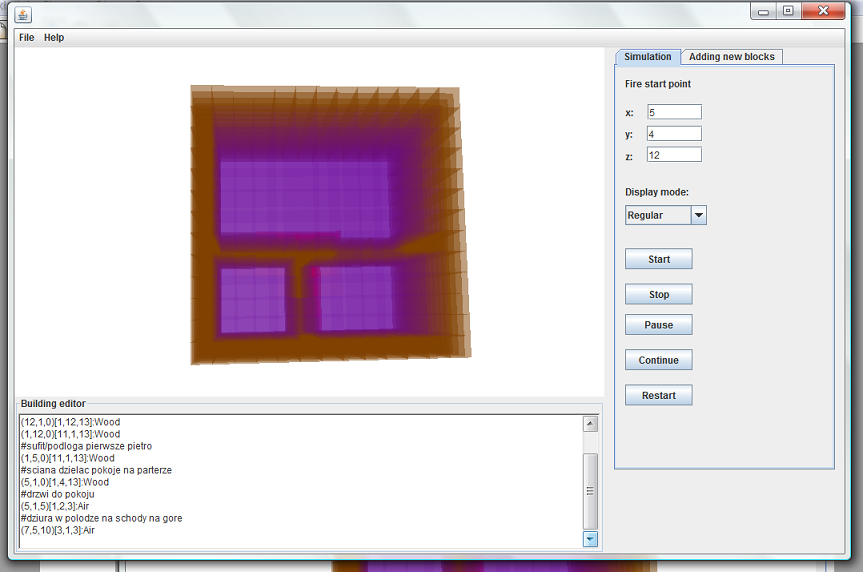
\includegraphics{gui_cale.png} 
\caption { Graficzny interfejs użytkownika}
\label {gui_cale}
\end{center}
\end{figure}
W celu zapewnienia wygody i efektywności pracy został podzielony na następujące części:
\begin {enumerate}
\item Panel górny
\item Widok scenmy
\item Menu boczne
\item Edytor
\end {enumerate}
\section{Panel górny}
Panel górny zawiera elementy:
\begin{itemize}
\item File, składający się z pozycji:
\begin{itemize}
\item Save cell states - zapis stanu komórek automatu do pliku. Automat zapisany jest w postaci zbioru macierzy dwuwymiarowych, z których każda przedstawia jeden poziom automatu począwszy od poziomu 0 zgodnie z osią Y.
\item Save temperatures - zapis rozkładu temperatur automatu. Format zapisu identyczny z przypadkiem stanu komórek.
\item Read building from file - możliwość wczytania budynku z pliku. Format zapisu budynku w pliku jest taki sam jak w edytorze.
	Po wczytaniu budynku z pliku, jego opis pojawia się w edytorze co pozwala na dalsze modyfikacje.
\end {itemize}
\item Help, skonstruowany z opcji:
\begin {itemize}
\item User guide - podstawowe informacje o użytkowaniu programu: jak korzystać z edytora oraz panelu bocznego.
\item About program - podstawowe informacje o programie.
\end {itemize}
\end{itemize}

\section{Scena}
Główny elementem interfejsu jest scena, przedstawiająca wyniki symulacji. Aplikacja dostarcza możliwość manipulowania sceną w celu zróżnicowania widoku. Możliwe są do wykonania następujące akcje:
\begin {itemize}
\item Oddalanie i przybliżanie sceny za pomocą strzałek klawiatury. Strzałka w górę powoduje przybliżenie, zaś strzałka w dół oddalenie.
\item Obrót elementów na scenie za pomocą strzałek w bok. Strzałka w prawo obraca scenę zgodnie z ruchem wskazówek zegara, zaś strzałka w lewo przeciwnie do ich ruchu.
\end {itemize}

\section{Edytor}
Elementem wykorzystywanym do edycji budynku jest umieszczony na dole interfejsu edytor.
Edytor, jak zostało to opisane w rozdziale \ref{cha:implementacja} jest polem tekstowym i jako takie umożliwia
 operacje zaznaczania, kopiowania, wklejania i usuwania tekstu za pomocą standardowych skrótów klawiaturowych.
 Tekts umieszczany w edytorze służy do konstrukcji budynku, w którym przeprowadzana jest symulacja pożaru i powinien być zgodny z następującym formatem:
 \begin{enumerate}
 \item Konieczne jest aby każdy element konstrukcyjny był zapisany w osobnej linii.
 \item Pojedynczy, dodawany element jest ortogonalnym, jednolitym blokiem o następującej postaci:
 \begin{center}
	(Start\_X,Start\_Y,Start\_Z)[Rozmiar\_X,Rozmiar\_Y,Rozmiar\_Z]:Material
 \end {center}
 gdzie:
	 \begin{itemize}
	 \item (Start\_X,Start\_Y,Start\_Z) - są to adekwatnie współrzędne (X,Y,Z) Lewego-Dolnego-Tylnego wierzchołka bloku, będącego początkiem bloku co przedstawia rysunek \ref{osie}. 
	 \item $[$Rozmiar\_X,Rozmiar\_Y,Rozmiar\_Z$]$ - określają rozmiar wprowadzanego bloku. 
	 \item Komórki w automacie numerwane są od 0. Wszystkie współrzędne są całkowitymi liczbami nieujemnymi i oznaczają wielokrotność komórek w danej osi.
	 \item Materiał jest nazwą jednego z dostępnych materiałów. Dostępne materiały to:
	 \begin {itemize}
	 \item Drewno
	 \item Metal
	 \item Cegła
	 \item Powietrze
	 \end {itemize}
	 Blok zbudowany z materiału powietrze, może być wykorzystany do wstawienia dziury w ścianie lub podłodze odpowiadającej oknu lub przejściu na wyższe piętro budynku.
	 \end{itemize}
\item Linia rozpoczynająca się od znaku # jest traktowana jako komentarz i nie podlega analizie.
 \end {enumerate}
 \begin{figure}
\begin{center}
\includegraphics{osie.jpg} 
\caption { Orientacja bloku}
\label {osie}
\end{center}
\end{figure}
\section{Panel boczny}
Panel boczny składa się z dwóch zakładek:
\begin {enumerate}
\item Zakładka \textit{Simulation} dostarcza opcje pozwalające kontrolować przebieg symulacji.
\begin {itemize}
	\item Trzy pola tekstowe oznaczone etykietami \textit{x},\itextit{y} i \textit{z} pozwalają podać współrzędne bloku, w którym rozpoczyna się pożar.
	\item Pole wyboru trybu \textit{Diplay mode} przełącza scenę w jeden z dwóćh trybów:
	\begin{itemize}
	\item Tryb regularny - domyślny tryb, w którym pokazany jest aktualny stan komórki. Komórka będą w stanie naturalnym zachowuje kolor i przeźroczystość materiału z którego została stworzona. Komórka paląca się ma kolor czerwony. Dym przedstawiony jest jako szary.
	\item Tryb temperaturowy - przedstawia rozkład temperatur w budynku. Kolor niebiskie oznacza temperaturę z zakresu $[20-50^\circ C]$. Temperatury powyżej $50^\circ C$ przedstawione są w odcieniach czerwieni. Im intensywniejsza czerwień, tym większa temperatura.
\end{itemize}
	\item Guziki \textit {Start}, \textit{Stop}, \textit{Pause}, \textit{Continue}, \textit {Restart} pozwalają na kontrolowanie symulacji. Umożliwiają na przykład zatrzymanie pracy automatu w celu zapisu wyników pośrednich lub modyfikacji budynku, a następnie wznowienie działania.
	\end{itemize}
\item Zakładka \textit{Adding new blocks} jest alternatywą \textit{Edytora}. Umożliwia edycję budynku i jest przydatna szczególnie dla osób nieobytych z tekstowymi narzędziami pracy. Omawiana zakładka składa się z:
\begin {itemize}
\item Pola umowżliwiającego wybór materiału dla dodawanego bloku.
\item Pól tekstowych pozwalających wpisać współrzędne punktu startu dodawanego bloku oraz jego rozmiar.
\item Przycisku \textit{Add}, którego kliknięcie powoduje zaakceptowanie wprowadzonych zmian i utworzenie bloku.
\end {itemize}
\end {enumerate}
 



% itd.
% \appendix
% \include{dodatekA}
% \include{dodatekB}
% itd.

\bibliography{bibliografia}

\end{document}

